\documentclass[12pt]{problemClass}
\font\myfont=cmr12 at 41pt
\title{{\myfont Cauchy Sequence}}
\date{07-08-2019}
\author{Claudiu Rediu}
\usepackage[margin=0.5in]{geometry}
\usepackage[utf8]{inputenc}
\usepackage[english]{babel}
\usepackage{amsthm}
\usepackage{amssymb}
\usepackage{amsmath}
\usepackage{graphicx}
\renewcommand\qedsymbol{$\blacksquare$}
\usepackage{float}
\theoremstyle{definition}
\newtheorem*{definition}{Definition} %the * is such that the definition are not numbered
\theoremstyle{theorem}
\newtheorem{theorem}{Theorem}

\begin{document}
	\pagenumbering{gobble}
	\maketitle
	\newpage
	\pagenumbering{arabic}
	\newpage
	\begin{figure}[h]
		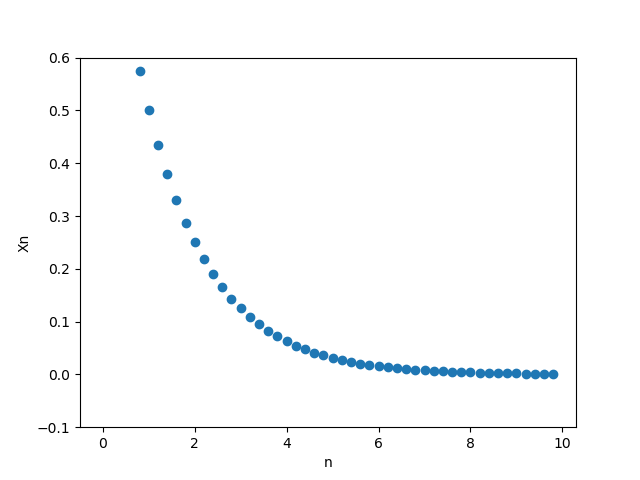
\includegraphics[width = \linewidth]{graph.png}
		\caption{Representation for the Cauchy Sequence $\{\frac{1}{2^x}\}$ }
	\end{figure}
	\begin{definition}{Cauchy Sequence}
		
		A sequence $\{a_n\}$ is called a \textbf{Cauchy Sequence} if for every $\epsilon > 0 $ there is a natural number $N$ such that, for all m and n, 
		$$ if \ m, n > N \ then \ |a_n - a_m| < \epsilon $$
		(This condition is usually written $\lim_{m,n \to +\infty} |a_m - a_n| = 0 $)
	\end{definition}
	
	\begin{theorem}
		A sequence $\{a_n\}$ converges if and only if it is a Cauchy sequence.
	\end{theorem}

	\begin{proof}
		The first part of the proof is satisfied by the Bolzano-Weierstrass Theorem (every bounded sequence has a convergent subsequence). What is needed to prove the converse assertion is that every Cauchy sequence $\{a_n\}$ is bounded.
		If we take $\epsilon = 1$ in the definition of a Cauchy sequence we find that there is some $N$ such that
		$$|a_m - a_n| < 1 \ for \ m,n > N $$
		In particular, this means that
		$$ |a_m - a_{N+1}| < 1 \ for \  all \ m > N$$
		Thus $\{a_m : m > N\}$ is bounded; since there are only finitely many other $a_i$s such that the whole sequence is bounded.
		Suppose that a subsequence of a Cauchy sequence converges. Taking into consideration that the difference between the elements of a Cauchy sequence is very small and some subsequence of it converges, then for every $\epsilon > 0$ there is a natural number $N$ such that, for all $m$ and $n$,
		$$ if \ m, n > N \ then \ |a_n - a_m| < \epsilon $$
	\end{proof}

	
\end{document}